% generated by Plantuml 1.2026.8
\definecolor{plantucolor0000}{RGB}{0,0,0}%
\definecolor{plantucolor0001}{RGB}{255,255,255}%
\definecolor{plantucolor0002}{RGB}{255,255,255}%
\definecolor{plantucolor0003}{RGB}{7,92,163}%
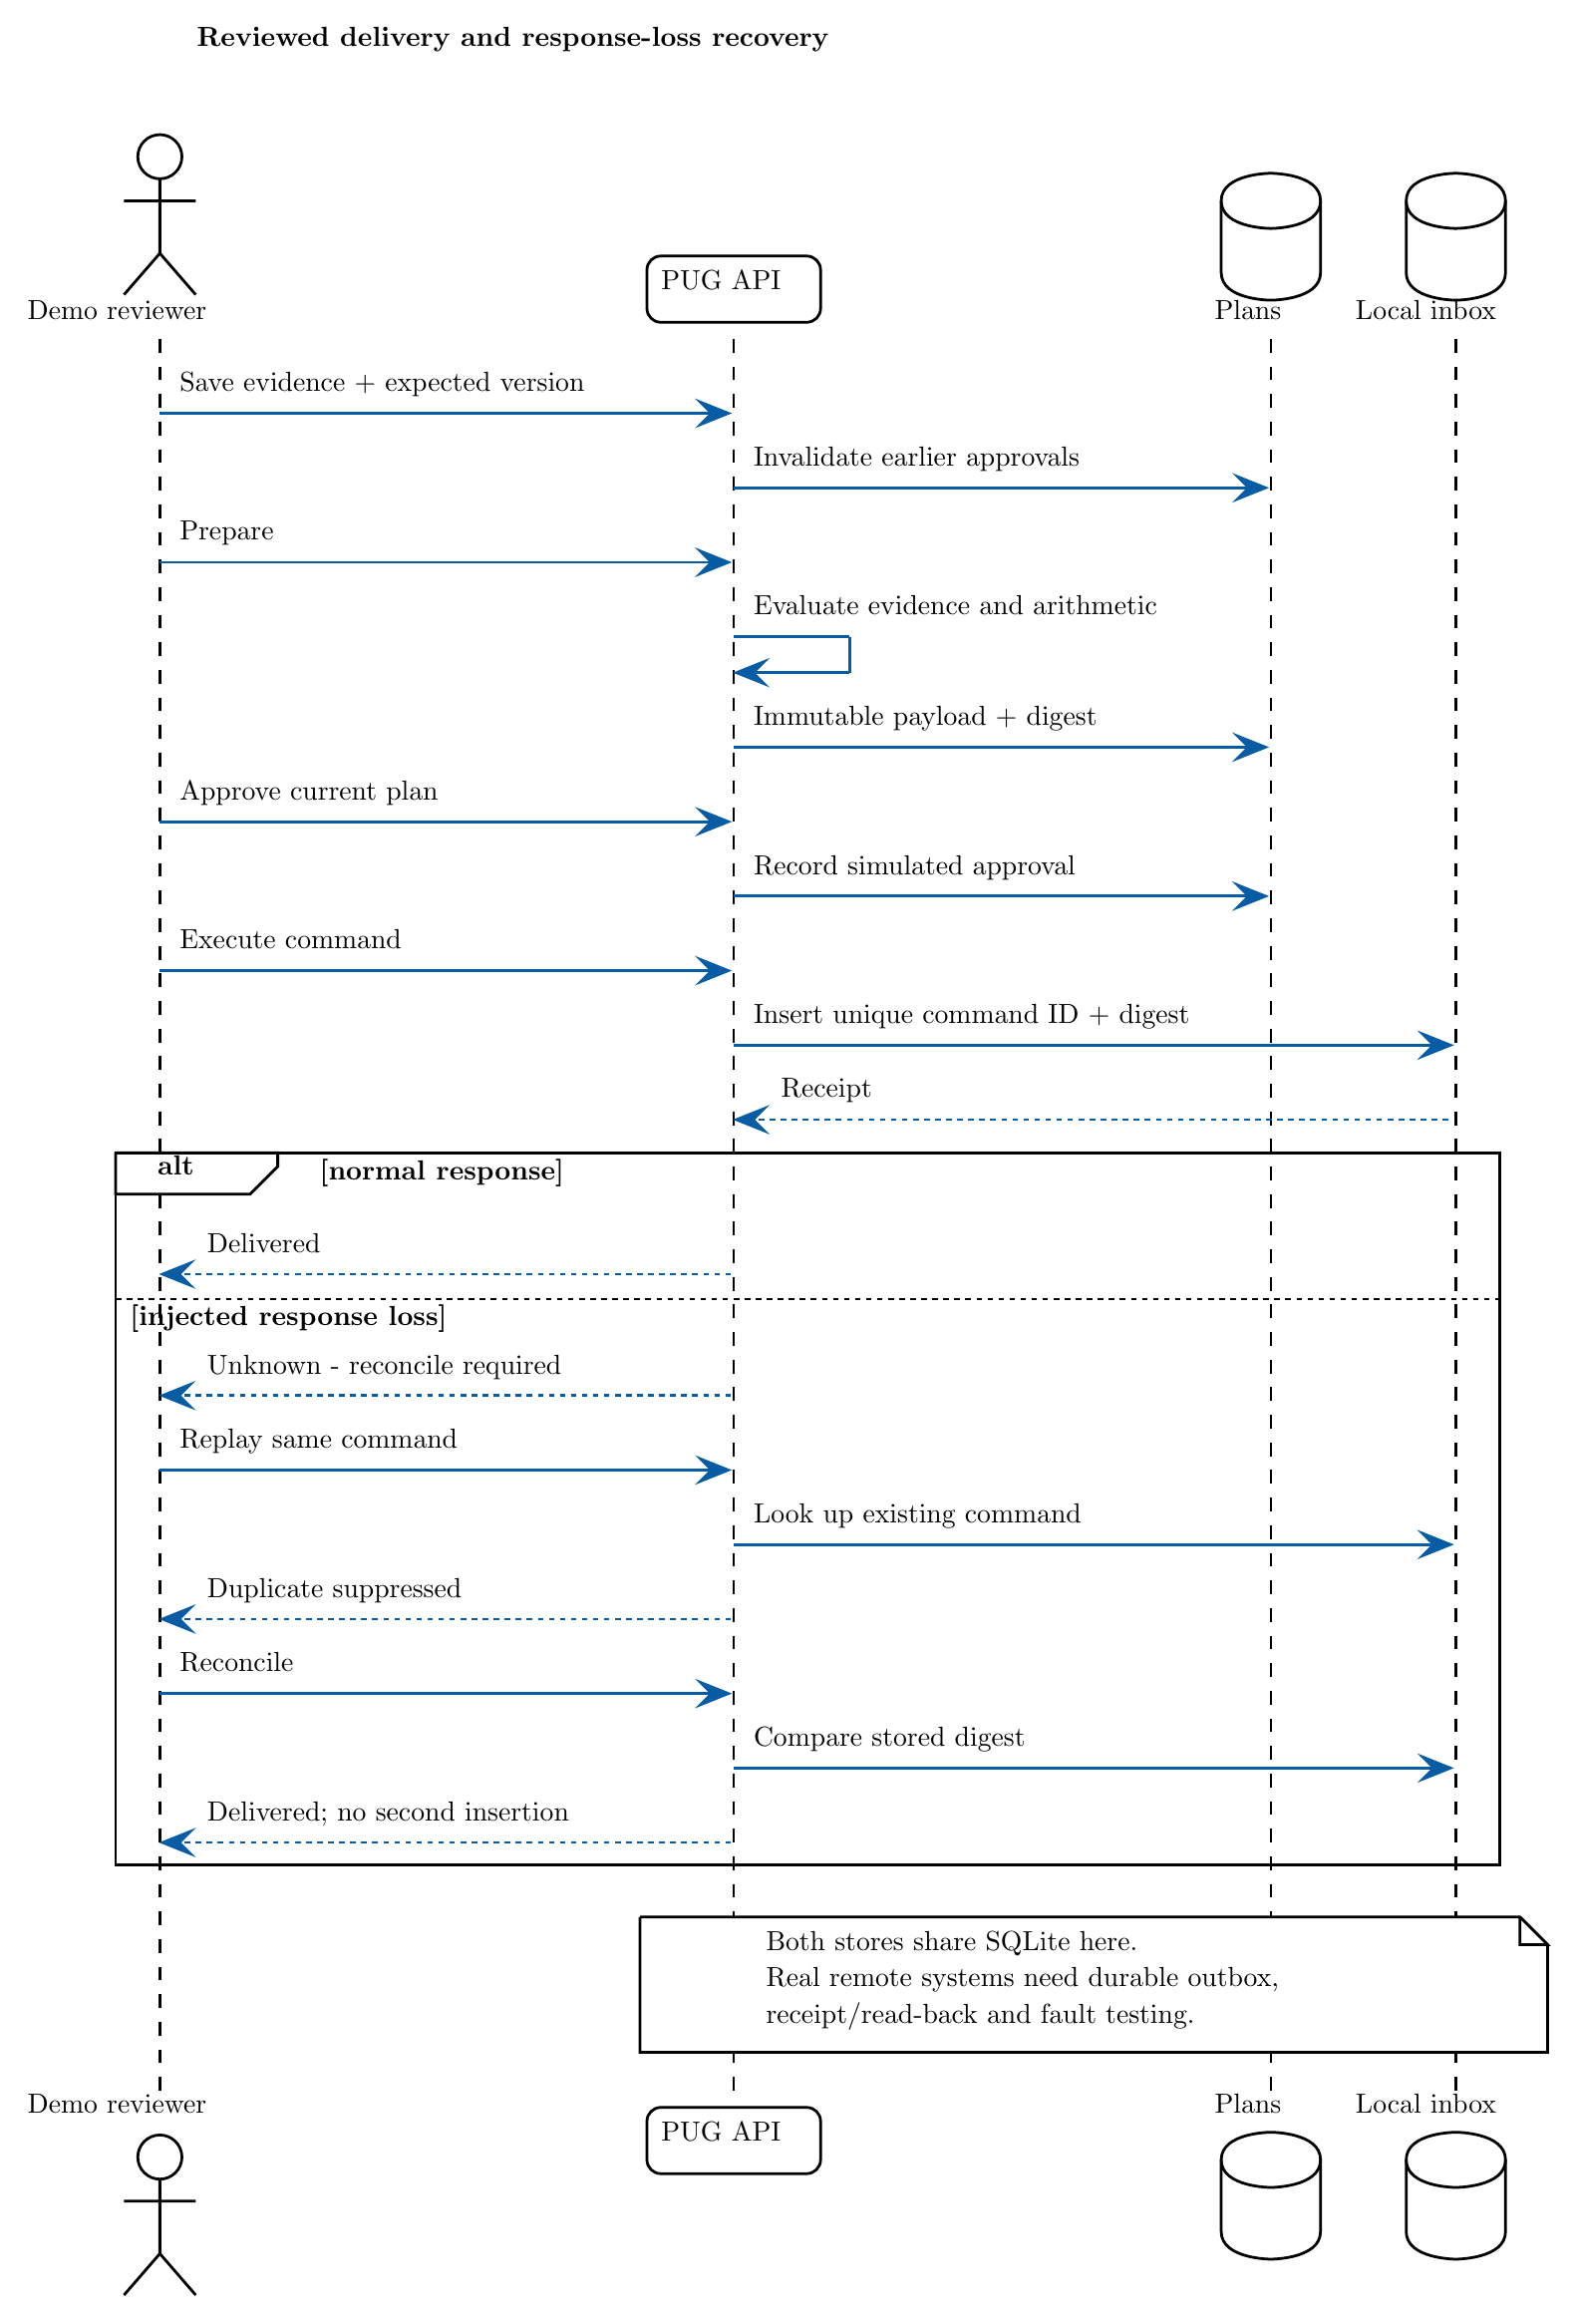
\begin{tikzpicture}[yscale=-1
,pstyle1/.style={color=black,line width=1.0pt}
,pstyle2/.style={color=plantucolor0002,line width=0.0pt}
,pstyle3/.style={color=black,line width=1.0pt,dash pattern=on 5.0pt off 5.0pt}
,pstyle4/.style={color=black,fill=white,line width=1.0pt}
,pstyle5/.style={color=plantucolor0003,fill=plantucolor0003,line width=1.0pt}
,pstyle6/.style={color=plantucolor0003,line width=1.0pt}
,pstyle7/.style={color=plantucolor0003,line width=1.0pt,dash pattern=on 2.0pt off 2.0pt}
]
\node at (71.4pt,15pt)[below right,color=black,inner sep=0]{\textbf{Reviewed delivery and response-loss recovery}};
\draw[color=white,fill=white,line width=1.0pt] (42.15pt,423pt) rectangle (543.9375pt,681pt);
\draw[pstyle1] (42.15pt,423pt) rectangle (543.9375pt,681pt);
\draw[pstyle2] (54.65pt,128pt) rectangle (62.65pt,764pt);
\draw[pstyle3] (58.15pt,128pt) -- (58.15pt,764pt);
\draw[pstyle2] (262.6813pt,128pt) rectangle (270.6813pt,764pt);
\draw[pstyle3] (266.1813pt,128pt) -- (266.1813pt,764pt);
\draw[pstyle2] (457.3813pt,128pt) rectangle (465.3813pt,764pt);
\draw[pstyle3] (460.8813pt,128pt) -- (460.8813pt,764pt);
\draw[pstyle2] (524.4375pt,128pt) rectangle (532.4375pt,764pt);
\draw[pstyle3] (527.9375pt,128pt) -- (527.9375pt,764pt);
\node at (10pt,114pt)[below right,color=black,inner sep=0]{Demo reviewer};
\draw[pstyle4] (58.15pt,62pt) ellipse (8pt and 8pt);
\draw[pstyle1] (58.15pt,70pt) -- (58.15pt,97pt)(45.15pt,78pt) -- (71.15pt,78pt)(58.15pt,97pt) -- (45.15pt,112pt)(58.15pt,97pt) -- (71.15pt,112pt);
\draw[pstyle4] (234.7125pt,103pt) arc (180:270:5pt) -- (239.7125pt,98pt) -- (292.65pt,98pt) arc (270:360:5pt) -- (297.65pt,103pt) -- (297.65pt,117pt) arc (0:90:5pt) -- (292.65pt,122pt) -- (239.7125pt,122pt) arc (90:180:5pt) -- (234.7125pt,117pt) -- cycle;
\node at (239.7125pt,103pt)[below right,color=black,inner sep=0]{PUG API};
\node at (440.3375pt,114pt)[below right,color=black,inner sep=0]{Plans};
\draw[pstyle4] (442.8813pt,78pt) ..controls (442.8813pt,68pt) and (460.8813pt,68pt) .. (460.8813pt,68pt) ..controls (460.8813pt,68pt) and (478.8813pt,68pt) .. (478.8813pt,78pt) -- (478.8813pt,104pt) ..controls (478.8813pt,114pt) and (460.8813pt,114pt) .. (460.8813pt,114pt) ..controls (460.8813pt,114pt) and (442.8813pt,114pt) .. (442.8813pt,104pt) -- (442.8813pt,78pt);
\draw[pstyle1] (442.8813pt,78pt) ..controls (442.8813pt,88pt) and (460.8813pt,88pt) .. (460.8813pt,88pt) ..controls (460.8813pt,88pt) and (478.8813pt,88pt) .. (478.8813pt,78pt);
\node at (491.425pt,114pt)[below right,color=black,inner sep=0]{Local inbox};
\draw[pstyle4] (509.9375pt,78pt) ..controls (509.9375pt,68pt) and (527.9375pt,68pt) .. (527.9375pt,68pt) ..controls (527.9375pt,68pt) and (545.9375pt,68pt) .. (545.9375pt,78pt) -- (545.9375pt,104pt) ..controls (545.9375pt,114pt) and (527.9375pt,114pt) .. (527.9375pt,114pt) ..controls (527.9375pt,114pt) and (509.9375pt,114pt) .. (509.9375pt,104pt) -- (509.9375pt,78pt);
\draw[pstyle1] (509.9375pt,78pt) ..controls (509.9375pt,88pt) and (527.9375pt,88pt) .. (527.9375pt,88pt) ..controls (527.9375pt,88pt) and (545.9375pt,88pt) .. (545.9375pt,78pt);
\node at (10pt,764pt)[below right,color=black,inner sep=0]{Demo reviewer};
\draw[pstyle4] (58.15pt,787pt) ellipse (8pt and 8pt);
\draw[pstyle1] (58.15pt,795pt) -- (58.15pt,822pt)(45.15pt,803pt) -- (71.15pt,803pt)(58.15pt,822pt) -- (45.15pt,837pt)(58.15pt,822pt) -- (71.15pt,837pt);
\draw[pstyle4] (234.7125pt,774pt) arc (180:270:5pt) -- (239.7125pt,769pt) -- (292.65pt,769pt) arc (270:360:5pt) -- (297.65pt,774pt) -- (297.65pt,788pt) arc (0:90:5pt) -- (292.65pt,793pt) -- (239.7125pt,793pt) arc (90:180:5pt) -- (234.7125pt,788pt) -- cycle;
\node at (239.7125pt,774pt)[below right,color=black,inner sep=0]{PUG API};
\node at (440.3375pt,764pt)[below right,color=black,inner sep=0]{Plans};
\draw[pstyle4] (442.8813pt,788pt) ..controls (442.8813pt,778pt) and (460.8813pt,778pt) .. (460.8813pt,778pt) ..controls (460.8813pt,778pt) and (478.8813pt,778pt) .. (478.8813pt,788pt) -- (478.8813pt,814pt) ..controls (478.8813pt,824pt) and (460.8813pt,824pt) .. (460.8813pt,824pt) ..controls (460.8813pt,824pt) and (442.8813pt,824pt) .. (442.8813pt,814pt) -- (442.8813pt,788pt);
\draw[pstyle1] (442.8813pt,788pt) ..controls (442.8813pt,798pt) and (460.8813pt,798pt) .. (460.8813pt,798pt) ..controls (460.8813pt,798pt) and (478.8813pt,798pt) .. (478.8813pt,788pt);
\node at (491.425pt,764pt)[below right,color=black,inner sep=0]{Local inbox};
\draw[pstyle4] (509.9375pt,788pt) ..controls (509.9375pt,778pt) and (527.9375pt,778pt) .. (527.9375pt,778pt) ..controls (527.9375pt,778pt) and (545.9375pt,778pt) .. (545.9375pt,788pt) -- (545.9375pt,814pt) ..controls (545.9375pt,824pt) and (527.9375pt,824pt) .. (527.9375pt,824pt) ..controls (527.9375pt,824pt) and (509.9375pt,824pt) .. (509.9375pt,814pt) -- (509.9375pt,788pt);
\draw[pstyle1] (509.9375pt,788pt) ..controls (509.9375pt,798pt) and (527.9375pt,798pt) .. (527.9375pt,798pt) ..controls (527.9375pt,798pt) and (545.9375pt,798pt) .. (545.9375pt,788pt);
\draw[pstyle5] (254.1813pt,151pt) -- (264.1813pt,155pt) -- (254.1813pt,159pt) -- (258.1813pt,155pt) -- cycle;
\draw[pstyle6] (58.15pt,155pt) -- (260.1813pt,155pt);
\node at (65.15pt,140pt)[below right,color=black,inner sep=0]{Save evidence + expected version};
\draw[pstyle5] (448.8813pt,178pt) -- (458.8813pt,182pt) -- (448.8813pt,186pt) -- (452.8813pt,182pt) -- cycle;
\draw[pstyle6] (266.1813pt,182pt) -- (454.8813pt,182pt);
\node at (273.1813pt,167pt)[below right,color=black,inner sep=0]{Invalidate earlier approvals};
\draw[pstyle5] (254.1813pt,205pt) -- (264.1813pt,209pt) -- (254.1813pt,213pt) -- (258.1813pt,209pt) -- cycle;
\draw[pstyle6] (58.15pt,209pt) -- (260.1813pt,209pt);
\node at (65.15pt,194pt)[below right,color=black,inner sep=0]{Prepare};
\draw[pstyle6] (266.1813pt,236pt) -- (308.1813pt,236pt);
\draw[pstyle6] (308.1813pt,236pt) -- (308.1813pt,249pt);
\draw[pstyle6] (267.1813pt,249pt) -- (308.1813pt,249pt);
\draw[pstyle5] (277.1813pt,245pt) -- (267.1813pt,249pt) -- (277.1813pt,253pt) -- (273.1813pt,249pt) -- cycle;
\node at (273.1813pt,221pt)[below right,color=black,inner sep=0]{Evaluate evidence and arithmetic};
\draw[pstyle5] (448.8813pt,272pt) -- (458.8813pt,276pt) -- (448.8813pt,280pt) -- (452.8813pt,276pt) -- cycle;
\draw[pstyle6] (266.1813pt,276pt) -- (454.8813pt,276pt);
\node at (273.1813pt,261pt)[below right,color=black,inner sep=0]{Immutable payload + digest};
\draw[pstyle5] (254.1813pt,299pt) -- (264.1813pt,303pt) -- (254.1813pt,307pt) -- (258.1813pt,303pt) -- cycle;
\draw[pstyle6] (58.15pt,303pt) -- (260.1813pt,303pt);
\node at (65.15pt,288pt)[below right,color=black,inner sep=0]{Approve current plan};
\draw[pstyle5] (448.8813pt,326pt) -- (458.8813pt,330pt) -- (448.8813pt,334pt) -- (452.8813pt,330pt) -- cycle;
\draw[pstyle6] (266.1813pt,330pt) -- (454.8813pt,330pt);
\node at (273.1813pt,315pt)[below right,color=black,inner sep=0]{Record simulated approval};
\draw[pstyle5] (254.1813pt,353pt) -- (264.1813pt,357pt) -- (254.1813pt,361pt) -- (258.1813pt,357pt) -- cycle;
\draw[pstyle6] (58.15pt,357pt) -- (260.1813pt,357pt);
\node at (65.15pt,342pt)[below right,color=black,inner sep=0]{Execute command};
\draw[pstyle5] (515.9375pt,380pt) -- (525.9375pt,384pt) -- (515.9375pt,388pt) -- (519.9375pt,384pt) -- cycle;
\draw[pstyle6] (266.1813pt,384pt) -- (521.9375pt,384pt);
\node at (273.1813pt,369pt)[below right,color=black,inner sep=0]{Insert unique command ID + digest};
\draw[pstyle5] (277.1813pt,407pt) -- (267.1813pt,411pt) -- (277.1813pt,415pt) -- (273.1813pt,411pt) -- cycle;
\draw[pstyle7] (271.1813pt,411pt) -- (526.9375pt,411pt);
\node at (283.1813pt,396pt)[below right,color=black,inner sep=0]{Receipt};
\draw[pstyle4] (42.15pt,423pt) -- (100.8813pt,423pt) -- (100.8813pt,428pt) -- (90.8813pt,438pt) -- (42.15pt,438pt) -- (42.15pt,423pt);
\draw[pstyle1] (42.15pt,423pt) rectangle (543.9375pt,681pt);
\node at (57.15pt,424pt)[below right,color=black,inner sep=0]{\textbf{alt}};
\node at (115.8813pt,425pt)[below right,color=black,inner sep=0]{\textbf{[normal response]}};
\draw[pstyle5] (69.15pt,463pt) -- (59.15pt,467pt) -- (69.15pt,471pt) -- (65.15pt,467pt) -- cycle;
\draw[pstyle7] (63.15pt,467pt) -- (265.1813pt,467pt);
\node at (75.15pt,452pt)[below right,color=black,inner sep=0]{Delivered};
\draw[color=black,line width=1.0pt,dash pattern=on 2.0pt off 2.0pt] (42.15pt,476pt) -- (543.9375pt,476pt);
\node at (47.15pt,478pt)[below right,color=black,inner sep=0]{\textbf{[injected response loss]}};
\draw[pstyle5] (69.15pt,507pt) -- (59.15pt,511pt) -- (69.15pt,515pt) -- (65.15pt,511pt) -- cycle;
\draw[pstyle7] (63.15pt,511pt) -- (265.1813pt,511pt);
\node at (75.15pt,496pt)[below right,color=black,inner sep=0]{Unknown - reconcile required};
\draw[pstyle5] (254.1813pt,534pt) -- (264.1813pt,538pt) -- (254.1813pt,542pt) -- (258.1813pt,538pt) -- cycle;
\draw[pstyle6] (58.15pt,538pt) -- (260.1813pt,538pt);
\node at (65.15pt,523pt)[below right,color=black,inner sep=0]{Replay same command};
\draw[pstyle5] (515.9375pt,561pt) -- (525.9375pt,565pt) -- (515.9375pt,569pt) -- (519.9375pt,565pt) -- cycle;
\draw[pstyle6] (266.1813pt,565pt) -- (521.9375pt,565pt);
\node at (273.1813pt,550pt)[below right,color=black,inner sep=0]{Look up existing command};
\draw[pstyle5] (69.15pt,588pt) -- (59.15pt,592pt) -- (69.15pt,596pt) -- (65.15pt,592pt) -- cycle;
\draw[pstyle7] (63.15pt,592pt) -- (265.1813pt,592pt);
\node at (75.15pt,577pt)[below right,color=black,inner sep=0]{Duplicate suppressed};
\draw[pstyle5] (254.1813pt,615pt) -- (264.1813pt,619pt) -- (254.1813pt,623pt) -- (258.1813pt,619pt) -- cycle;
\draw[pstyle6] (58.15pt,619pt) -- (260.1813pt,619pt);
\node at (65.15pt,604pt)[below right,color=black,inner sep=0]{Reconcile};
\draw[pstyle5] (515.9375pt,642pt) -- (525.9375pt,646pt) -- (515.9375pt,650pt) -- (519.9375pt,646pt) -- cycle;
\draw[pstyle6] (266.1813pt,646pt) -- (521.9375pt,646pt);
\node at (273.1813pt,631pt)[below right,color=black,inner sep=0]{Compare stored digest};
\draw[pstyle5] (69.15pt,669pt) -- (59.15pt,673pt) -- (69.15pt,677pt) -- (65.15pt,673pt) -- cycle;
\draw[pstyle7] (63.15pt,673pt) -- (265.1813pt,673pt);
\node at (75.15pt,658pt)[below right,color=black,inner sep=0]{Delivered; no second insertion};
\draw[pstyle4] (232.1906pt,700pt) -- (232.1906pt,749pt) -- (561.1906pt,749pt) -- (561.1906pt,710pt) -- (551.1906pt,700pt) -- (232.1906pt,700pt);
\draw[pstyle4] (551.1906pt,700pt) -- (551.1906pt,710pt) -- (561.1906pt,710pt) -- (551.1906pt,700pt);
\node at (277.7125pt,705pt)[below right,color=black,inner sep=0]{Both stores share SQLite here.};
\node at (277.7125pt,718pt)[below right,color=black,inner sep=0]{Real remote systems need durable outbox,};
\node at (277.7125pt,731pt)[below right,color=black,inner sep=0]{receipt/read-back and fault testing.};
\end{tikzpicture}%
